%% HEADER
%%%%%%%%%%%%%%%%%%%%%%%%%%%%%%%%%%%%%%%%%%%%%%%%%%%%%%%%%%%%%
\newcommand{\hyperrefpdfauthor}{Konstantin Manna}
\newcommand{\hyperrefpdftitle}{Robust wireless link and channel assignment algorithm minimizing interference utilizing multi-radio access points}
\newcommand{\hyperrefpdfsubject}{Bachelor Thesis}
\newcommand{\hyperrefpdfkeywords}{}
\newcommand{\hyperrefpdfborder}{0}
\documentclass{styles/wissdoc-kw-eng}

\usepackage{subfigure}

\usepackage{hyperref}
\usepackage{acronym}
\renewcommand{\bflabel}[1]{\normalfont{\normalsize{#1}}\hfill} % keine serifenlose schrift für acronym

\usepackage{float}
\floatstyle{ruled}
\newfloat{listing}{htbp}{lop}[chapter]
\floatname{listing}{Listing}

\usepackage[hang,center,nooneline]{caption}
\captionsetup[figure]{font={small,sf}}
%\captionsetup[table]{font={small,sf}}
\captionsetup[listing]{font={small,sf}}
\usepackage{etoolbox}


%% Normales LaTeX oder pdfLaTeX? %%%%%%%%%%%%%%%%%%%%%%%%%%%%
%% ==> Das neue if-Kommando "\ifpdf" wird an einigen wenigen
%% ==> Stellen benötigt, um die Kompatibilität zwischen
%% ==> LaTeX und pdfLaTeX herzustellen.
%\newif\ifpdf
%\ifx\pdfoutput\undefined
%    \pdffalse              %%normales LaTeX wird ausgeführt
%\else
%    \pdfoutput=1
%    \pdftrue               %%pdfLaTeX wird ausgeführt
%\fi


%% Fonts für pdfLaTeX %%%%%%%%%%%%%%%%%%%%%%%%%%%%%%%%%%%%%%%
%% ==> Nur notwendig, falls keine cm-super-Fonts installiert
\ifpdf
	\usepackage{ae}       %%Benutzen Sie nur eines dieser Pakete:
	%\usepackage{zefonts}  %%je nachdem, welches Sie besitzen.
\else
	%%Normales LaTeX - keine speziellen Fontpackages notwendig
\fi


%% Deutsche Anpassungen %%%%%%%%%%%%%%%%%%%%%%%%%%%%%%%%%%%%%
%\usepackage[T1]{fontenc}
%\usepackage[utf8]{inputenc}

%% zur Zitaten des Quelltextes%%%%%%%%%%%%%%%%%%%%%%%%%%%%%%%
% "final" forces printing of all listings, even if the global "draft" is set
\usepackage[final]{listings}
\lstset{
    basicstyle=\footnotesize\ttfamily,
    tabsize=4,
    numberstyle=\tiny\color{gray},
    numbersep=5pt,
    numbers=left,
    captionpos=b,
    abovecaptionskip=0pt,
    belowcaptionskip=0pt,
    aboveskip=10pt,
    belowskip=0pt,
    floatplacement=tbp,
    frame=topline,
    framerule=.1pt,
    framesep = 3pt,
    }
\renewcommand\lstlistingname{\textbf{Listing}}
% This is only kept for backwards compatibility. You should never have to use it. Use the listing-environment instead.
%\DeclareCaptionFormat*{lstruled}{{\bfseries#1\small\space\normalfont#3\hrule height.1pt depth0pt}\par}
%\captionsetup[lstlisting]{format=lstruled,singlelinecheck=false}

%% mehrere Abbildungen in eine %%%%%%%%%%%%%%%%%%%%%%%%%%%%%%
\usepackage{subfigure}

%% Packages für Formeln %%%%%%%%%%%%%%%%%%%%%%%%%%%%%%%%%%%%%
\usepackage{amsmath}
\usepackage{amsthm}
\usepackage{amsfonts}

%% Zeilenabstand %%%%%%%%%%%%%%%%%%%%%%%%%%%%%%%%%%%%%%%%%%%%
\usepackage{setspace}
%\singlespacing        %% 1-zeilig (Standard)
%\onehalfspacing       %% 1,5-zeilig
%\doublespacing        %% 2-zeilig


%% Andere Packages %%%%%%%%%%%%%%%%%%%%%%%%%%%%%%%%%%%%%%%%%%
%\usepackage{a4wide} %%Kleinere Seitenränder = mehr Text pro Zeile.
\usepackage{fancyhdr} %%Fancy Kopf- und Fußzeilen
%\usepackage{longtable} %%Für Tabellen, die eine Seite überschreiten
\usepackage{lscape}
\usepackage{rotating} 
%\usepackage[htt]{hyphenat} %Trennung von Typewriter-Schriften
%\usepackage{listings}
\usepackage{pstricks-add}


% Tabellen mit Center und left
\usepackage{tabularx,colortbl} % colored table background
\newcolumntype{C}[1]{>{\centering\arraybackslash}p{#1}}
\newcolumntype{R}[1]{>{\raggedleft\arraybackslash}p{#1}}
% Table spacings
\newcommand\T{\rule{0pt}{2.5ex}\rule[-1.0ex]{0pt}{0pt}}
\newcommand\B{\rule[-1.0ex]{0pt}{0pt}}

\definecolor{slightgray}{gray}{.90} 


%% Definitionen %%%%%%%%%%%%%%%%%%%%%%%%%%%%


%% zur Benutzung bei ergänzenden Daten%%%%%%%%%%%%%%%%%%%%%%%%
%\usepackage{endnotes}
%\renewcommand{\notesname}{Konfigurationsdaten der Messreihen}
%\renewcommand{\theendnote}{\Alph{endnote}}
%\renewcommand{\enotesize}{\normalsize}

%\hyphenation{Sensor-netz-werk
%}

%%%%%%%%%%%%%%%%%%%%%%%%%%%%%%%%%%%%%%%%%%%%%%%%%%%%%%%%%%%%%
%% DOKUMENT
%%%%%%%%%%%%%%%%%%%%%%%%%%%%%%%%%%%%%%%%%%%%%%%%%%%%%%%%%%%%%
\begin{document}

%% Dateiendungen für Grafiken %%%%%%%%%%%%%%%%%%%%%%%%%%%%%%%
%% ==> Sie können hiermit die Dateiendung einer Grafik weglassen.
%% ==> Aus "\includegraphics{titel.eps}" wird "\includegraphics{titel}".
%% ==> Wenn Sie nunmehr 2 inhaltsgleiche Grafiken "titel.eps" und
%% ==> "titel.pdf" erstellen, wird jeweils nur die Grafik eingebunden,
%% ==> die von ihrem Compiler verarbeitet werden kann.
%% ==> pdfLaTeX benutzt "titel.pdf". LaTeX benutzt "titel.eps".
%\ifpdf
%    \DeclareGraphicsExtensions{.pdf,.jpg,.png}
%\else
%    \DeclareGraphicsExtensions{.eps}
%\fi

\pagestyle{empty} %%Keine Kopf-/Fusszeilen auf den ersten Seiten.

\ifnotdraft{
%% Deckblatt %%%%%%%%%%%%%%%%%%%%%%%%%%%%%%%%%%%%%%%%%%%%%%%%
\frontmatter
\titlehead{
	\centering
	\includegraphics[height=20mm,keepaspectratio]{logos/comsys-text}
	\hfill
	\includegraphics[height=20mm,keepaspectratio]{logos/rwth}
} % end titlehead

\begin{titlepage}

\let\footnotesize\small \let\footnoterule\relax

\hbox{}
\vfill

\centering

\begin{doublespace}
{ \huge\textbf{\textsf{Robust Wireless Link and Channel Assignment Algorithm
Minimizing Interference Utilizing Multi-Radio Access Points 
}}}
%{ \huge\textbf{\textsf{Your Awesome Thesis Title \\ \vspace{-0.4em}
%(Which May Also Be Long \\ \vspace{0.4em}
%And Stretch multiple Lines) Here}}}
\end{doublespace}
\vskip 2cm

{\large Bachelor Thesis\\[5pt]}
{\large \textbf{Konstantin Manna}}
\vskip 1cm

\textbf{RWTH Aachen University, Germany\\[5pt]
        Chair of Communication and Distributed Systems}
\vskip 2cm

\large

Advisors:
\vskip 2mm

\begin{tabular}{R{7cm}p{7cm}}
Dipl.-Inform. & Christoph Wollgarten\\
Dipl.-Inform. & J\'o \'Agila Bitsch Link\\
Prof.~Dr.-Ing. & Klaus Wehrle\\
Prof.~Dr. & Bernhard Rumpe
\end{tabular}
\vskip 1cm

\begin{tabular}{R{6cm}p{6cm}}
Registration date:  & 2014-05-20 \\
Submission date:    & 2014-09-22 \\
\end{tabular}

\vfill

\end{titlepage}


\cleardoublepage
\thispagestyle{empty}
\vspace*{36\baselineskip}
\hbox to \textwidth{\hrulefill}

I hereby affirm that I composed this work independently and used no other than the specified sources and tools and that I marked all quotes as such.

Hiermit versichere ich, dass ich die Arbeit selbstständig verfasst und keine anderen als die angegebenen Quellen und Hilfsmittel benutzt sowie Zitate kenntlich gemacht habe.

Aachen, den 2. März 2011

\cleardoublepage
\cleardoublepage

\chapter*{Acknowledgments}

I would like to thank Christoph Wollgarten at LANCOM for enabling and supervising this thesis, who despite his huge workload always had a few minutes to spare
to help me with my problems and create the AutoWDSstatus tool, which was much appreciated.
I also want to thank J\'o \'Agila Bitsch for supervising this thesis at COMSYS and his great feedback on this work during several meetings.
Furthermore i want to express my gratitude to Paul Smith who had some tipps and templates for writing this thesis.
Last but not least I thank Prof. Wehrle and Prof. Rumpe for giving me the chance to to write this thesis.
\cleardoublepage
\cleardoublepage

\vspace {2cm}
\begin{center}
\paragraph{Abstract}
\hrulefill
\end{center}
Using a wireless backbone in a \ac{WDS} can be tricky as performance decreases with increasing size due to interference if 
channels and network topology are not selected carefully beforehand. Additionally network dissociations may occur easily if 
crucial links fail as redundancy is neglected.

Therefore we present an algorithm and its implementation which addresses this problem by finding a network topology and channel assignment 
that minimizes interference and thus allows a deployment to increase its throughput performance by utilizing more bandwidth in the local spectrum. 
Our evaluation results show an increase in throughput performance of up to 9 times or more compared to a baseline scenario where an optimization has not taken place
and only one channel for the whole network is used.
Furthermore our solution also provides a robust network topology which tackles the issue of network partition for single link failures by using survival paths.

We achieve this gain in performance by utilizing multi-radio accesspoints and enhancing the \ac{DJP}-algorithm for graphs by a scoring system combined with
a greedy channel assignment.


\cleardoublepage

% Titelseite hatte noch normale Tabellen. Von hier ab sollen alle
% Tabellen laut style-Vorgaben sans serif sein.
\AtBeginEnvironment{tabular}{\sffamily}
\AtBeginEnvironment{tabularx}{\sffamily}

%% Inhaltsverzeichnis %%%%%%%%%%%%%%%%%%%%%%%%%%%%%%%%%%%%%%%
\tableofcontents %Inhaltsverzeichnis
\cleardoublepage %Das erste Kapitel soll auf einer ungeraden Seite beginnen.
} % end ifnotdraft

\pagestyle{fancy} %%Ab hier die Kopf-/Fusszeilen: headings / fancy / ...

%%%%%%%%%%%%%%%%%%%%%%%%%%%%%%%%%%%%%%%%%%%%%%%%%%%%%%%%%%%%%
% einzelne Kapitel
%%%%%%%%%%%%%%%%%%%%%%%%%%%%%%%%%%%%%%%%%%%%%%%%%%%%%%%%%%%%%
%\include{commands}

\mainmatter
\chapter{Introduction}
  The rise of smartphones and other devices that are capable of using IEEE 802.11 \ac{WLAN} bring along 
  more applications that exhaust any way to reconnect to the internet in order to 
  down an up-load personal data, advertisement or media with a high footprint in storage.
  YouTube, WhatsApp, Facebook and similar apps move high quality images and videos to and from end-users smartphones. 
  Since the number of smartphones in the field are constantly on the rise, this creates an additional strain for
  the backbone and access-links. As users prefer to use WLANs instead of mobile internet-connections due to their costs and limitations with respect to available bandwidth,
  a \ac{WLAN} infrastructure like a \ac{WDS} needs careful planning. Especially use cases like camping sites or large scale deployments (widespread rural areas) with a lot of users
  put high requirements on the \ac{WLAN} backbone. 
  In this paper we consider LANCOM \textit{AutoWDS}, a \ac{WDS} which implements an easily deployable \ac{WDS} for a set of APs in order to create a wireless 
  infrastructure for a specific area.

  \begin{figure}[h]
    \centering
    \includegraphics[width=1\columnwidth]{figures/camping.png}
    \caption{WDS deployment at a camping site. Typical scenario for using a \ac{WDS} system instead of wired APs.}
    \label{fig:camping}
  \end{figure}
  
\section{Motivation}
  \textit{AutoWDS} in its current form does not scale well as throughput performance and an increasing number of connectivity failures quickly bring the system to its limits.
  Our goal is to optimize this system by boosting throughput performance and decreasing the number of occurring simple link failures.
  We want to achieve this by utilizing multiple radios, channels and redundant links (survival paths) for establishing connections among the APs, as using only a single
  channel places artificial limits on the achievable bandwidth.
  This means also we only deal with the physical connectivity (link layer) and are independent of a routing system, which could be placed on top of our solution.
  The problem we face doing this and that our work will elaborate on is that a good selection of links and channels is not trivial even for a moderately sized scenario.
  To tackle this challenge we use centrally run greedy algorithms to give us a better solution to our problem for a static environment.
  
\section{Structure of Thesis}
  At first we will recall terms and concepts used in this work followed by taking a look at the requirements and restrictions a possible solution would have to deal with.
  In Chapter 4, we will then review related work on this field and outline why those approaches have not been pursued.
  Subsequently we will describe our algorithms for choosing a topology, creating backup links and the successive channel assignment, ensued by the implementation of 
  the aforementioned. We will also give an example on how to run the algorithms yourself for a simple scenario.
  In Chapter 7 the procedure is evaluated as a whole in practice and compared to the basic version of \textit{AutoWDS}.
  Finally we conclude our findings by portraying open issues and identifying promising approaches to pursue.

\chapter{Background}
General discription of used terms/systems in wikipedia like style. This means the description should not be too extensive.
And refer to further papers for more extensive descriptions.
\section{Wireless Networks}
  \subsection{WLAN Channel}
    %https://de.wikipedia.org/wiki/Wireless_LAN#Frequenzen\newline
    \begin{description}
    \item[What is a Channel?]
    \item[Overview on useable frequencies]
    \item[Interference]
    \item[Hidden Station Problem]
    \item[CSMA-CD/CA]
    \item[Analogy switch - collision domain]
    \end{description}
  \subsection{Wireless Access-Point}
    %Used to establish wireless connections to devices, like laptops/mobile phones, but also printer and ... 
    %Connecting wired LAN - wireless LAN \newline
    %Mostly provide access to internet\newline
    %Usecases of Accesspoints\newline
    %https://de.wikipedia.org/wiki/Wireless_Access_Point \newline
  \subsection{Wireless Mesh Network}
    %https://de.wikipedia.org/wiki/Ad-hoc-Netz
    %Topology for nodes(devices) in a wireless network.
    %Self healing capabilities.
    %Role of Mesh routers.
    %Redundancy in mesh networks.
    %Autonomy of devices.
    %Infrastructure mode vs p2p mode
    %IEEE 802.11
    %Alterations in our scenario compared to standard mesh\newline
    \cite{Akyildiz2005445}
    \cite{airberry}
    \subsection{Wireless Distribution System}
    %https://en.wikipedia.org/wiki/Wireless_distribution_system
    Description of WDS + AutoWDS \newline
      \begin{description}
       \item[What is a Wireless Distribution System?]
       \item[How does the Lancom AutoWDS differ from the basic WDS definition?]
	 Intended centralized solution compüared to WDS systems due to better managability.
	 Also security is a key element for this system => that's why central entity + CAPWAP
      \end{description}
      \subsection{VLAN}
      \subsection{Spanning Tree + STP}
      \subsection{bandwidth}
      \subsection{BFS}
      \subsection{OpenVZ}
	\cite{openvz}
\section{Graph-theoretic Basics}
  %https://de.wikipedia.org/wiki/Graph_%28Graphentheorie%29
  TODO: Describe directed/undirected weighted graph
  What does connected graph mean; path
   \subsection{Mapping Data to Graph}
    For our solution we will use the following mapping from devices and modules to a undirected, weighted graph. (Formale beschreibung hilfreich?)
    Each accesspoint and each module of those accesspoints is represented by a node.
    For each accesspoint we add edges with the highest weight to each module of its corresponding accesspoint. 
    We describe those edges as artificial or device-module edges.
    If two modules of different accesspoints are within receive range of each other, 
    we are adding an edge between the corresponding module nodes with the average signal-to-noise ratio as the edge-weight.
    We call those edges module-module connections or real connections.
    Since the average of the two SNR's might not adequately represent the actual quality of those connections,
    we alternatively can easily adjust the edge-weight to the minimum or maximum of those values.
    While the average seems to be a good compromise for a general description of the underlying network, the minimum might be a better representation for 
    a more pessimistic setup, since the connection is then guaranteed to have at least this SNR in both directions. 
    Furthermore we are ignoring onesided connections, i.e. one module receives one or a few beacons of the other module but not the other way round.
    Not only are the SNRs of those connections mostly very poor, but they are also very rare in our target scenarios with omnidirectional antennas.
    So mostly either the modules receive each others beacons, or both do not.
    \begin{figure}[t]
      \centering
      \includegraphics[width=0.5\columnwidth]{figures/apgraph.png}
      \caption{Graph representation of one and two connected accesspoints}
      \label{fig:apgraph}
    \end{figure}
   \subsection{Relevance of COLORING}
   \subsection{Dijkstra's Algorithm}
   TODO: How is our Channel assignment related to the problem COLORING?
    It is realated in the way that we want to assign each Module-Module-Connection a channel/color from a pool of available colors, withouth (if possible) use the same channel/color on neighboring links (meaning Aps that see each other and their traffic could lead to decreased throughput due to interference)
    Why is it not just coloring?

\chapter{Requirement Analysis}
General answer to question of feasibility
  \section{Increase Throughput}
  Has to maximize overall throughput\newline
  \section{Reduce Network Connectivity Failures}
\section{Utilize variable Number of Radios}
  Should utilize multiple Radios per AP\newline
  Currently homogenous 2, Later 3, sometimes just 1 \newline
  Also should be able to handle heterogenous environments with respect to number of equipped radios \newline
\section{Restrictions}
  \subsection{Centralized Computation}
    Run on central entity (WLC), not distributed \newline 
  \subsection{Static Environment}
    System is only used for static environments (APs are not mobile) \newline
\section{Economical Restrictions}
  Ressource restrictions (Processing Power limited) \newline
  Duration (Results have to be available in limited time) \newline

\chapter{Related Work}
  The following four approaches are all solutions that are graph-based and target a centralized and static channel assignment.
  Those are not the only ones on this matter, but the most known and relevant contestants to our problem.
  Note that there are also numerous solutions on distributed and/or dynamic or semi-dynamic environments, which we will not covere here.
  Except the BFS-CA, the prevalent solutions make excessive use of the conflict graph, which according to \cite{overview_caa} has difficulties to model 
  the varying number of radios equipped on accesspoints. Also most of the works solely focus on assigning channels to an existing topology and do not touch 
  the network topology at all, what seems like a handicap as topology control is an essential part in dealing with wireless interference.
  
  \begin{figure}[h!]
    \centering
    \includegraphics[width=1\columnwidth]{figures/unit-disk-graph}
    \caption{Creation of an unit disk graph from the receive range map of accesspoints}
    \label{fig:unit-disk-graph}
  \end{figure}
  
  \section{\ac{CLICA}}
    The aim of \ac{CLICA} \cite{CLICA} is to minimize interference conflicts for a given unit disk graph preserving the connectivity.
    That means it takes the given network topology-graph as granted and tries to minimize the overall interference by resolving conflicts as much as possible.
    It takes the following parameters as input:
    
    \begin{itemize}
      \item Unit disk graph
      
      \item Number of radios at each node and total number of channels available
      
      \item Interference conflicts in form of a conflict graph
    \end{itemize}
    
    CLICA's mode of operation is described by \cite{overview_caa} as follows:
    \begin{itemize}
      \item Randomly assign a node \(v\) the highest priority, then assign other
	nodes priorities decreasing in the order obtained by depth.
	
      \item While traversing the nodes in the decreasing order of their
	priorities obtained above, assign channels to the incident links
	of these nodes. The operation of assigning a channel to a link
	includes assigning this channel to both a radio at this node and
	a radio at the neighbor node. Then, the priorities of unvisited
	nodes are adjusted according to their degree of flexibility, which
	is the number of channels that a node can choose from without
	breaking the connectivity preservation. Essentially, the nodes
	with a lower degree of flexibility will have their priorities
	increased so that they are visited earlier in the later steps.
	
      \item When picking a channel in the above step, a node v1 picks
	a channel for its incident link (\(v_1\) , \(v_2\) ) in a greedy manner: a
	locally optimal choice is made by selecting the channel that
	minimizes the maximum link conflict weight among all links
	that can interfere with link (\(v_1\) , \(v_2\) ). After a channel is assigned
	to a link, the conflict graph is updated to reflect the new link conflict weights.
    \end{itemize}
  
    The reason why we decided not to use this algorithm is that \ac{CLICA} only tries to minimize interference by assigning channels the best way possible for a given
    unit disk graph, which is basically each possible connection. For a highly connected network topology like \ref{fig:graphseen} this would lead to suboptimal results
    as it does not restrict itself to necessary connections and therfore possesses a lot of potential for interference.
    The restriction to use only the best and absolutely neccessary links is a vital part in order to 
    further decrease interference as much as possible for such a topology.
    
  \section{\ac{INSTC}}
    As pointed out by \cite{overview_caa}, INSTC \cite{INSTC} is similar to \ac{CLICA} with a few alterations, 
    which is why we will not go into further detail and rather focus on its differences. 
    They introduce \ac{LCI} which for a link represents the number of links which interfere with this link \cite{overview_caa} and serves as a measure of 
    interference. Additionally they accept \(k\) as input parameter which results in a \(k\)-connected Graph as outcome to make the topology resilient to node failures.
    Although this feature would come in handy for our survival path requirement, it does not match our failing scenario of a single link at a time instead of a whole node outage.
    Using a \textit{k}-(node)-connected graph instead of an \textit{k}-edge-connected graph increases the the number of edges that have to be utilized 
    (since one failing node involves several failing edges). Consequently the resulting network topology has a higher grade of connectivity than it needs to 
    have and therefore conversely affects overall throughput since a higher node connectivity leads to fewer useable different channels. 
    Additional to the weaknesses of \ac{CLICA}, they also require the number of radio modules per accesspoint to be identical, 
    which is not desireable for us as requirement analysis dictates the operability also for heterogenous networks where this
    restriction is not met. The LCI measure introduced in the work by \cite{INSTC} served as a basis for our edgescore calcuation in ~\ref{eq:edgescore}.
    
  \section{\ac{BFS-CA}}
    \ac{BFS-CA} \cite{BFS-CA} extends the common conflict graph with modules, resulting in a \ac{MCG} graph, which more closely reassembles the
    real world setup. This made it easier for them to deal with the different numbers of radios available on each accesspoints. 
    What they do is to let the accesspoints (or mesh routers in their case) sniff the network on regular intervalls and determine a ranking for the channels.
    Those rankings are then sent to their central entity, the \ac{CAS}. This \ac{CAS} in turn derives the \ac{MCG} and assigns each node in this graph 
    a channel in \ac{BFS}-manner by considering the received rankings of the accesspoints. In order not to partition the network by introducing a \ac{CA}, which 
    would disconnect some links by setting certain radios to different channels, they also use one radio on each accesspoint on an overall-common channel.
    This common channel is then used for initial setup, management frames and as a backup if other links break in order to keep the graph connectivity attribute.
    
    Although \ac{BFS-CA}, as others, is still anxious about topology alterations, since on a first glance it might introduce too severe problems like, 
    additional hops for packets, increased interference footprint and higher susceptibility to errors due to longer travel times of packets.
    Nevertheless it is the algorithm which we were inspired by the most and therefore have some ideas in common.
    The interesting features we reused and refined are:
    
    \begin{itemize}
     \item Idea of a ranking system for each possible channel
     
     \item Central computation on a \ac{CAS}, which reassembles our \ac{WLC}
     
     \item Taking foreign sources of interference also into consideration, instead of just internal.
     
    \end{itemize}
    
    Yet, we decided against its implementation for our purposes for the following reasons:
    
    \begin{itemize}
      \item Using all possible channels in the network topology creates to much interference for networks with more traffic.
	A selection process on this underlying topology is essential to our minds as selecting a few but high quality links
	leading to a planned and controlled topology will create a lot less interference than a network topology where all possible 
	links are used for communications. This is especially the case if not many channels are available for assignment, since 
	these can be more effectively designed (See \ref{fig:high_con_vs_low_con}).
	
      \item Using one radio on each accesspoint for a common overall-channel seemed to us as a waste of radio moduels.
	Radio modules on accesspoints are scarce and should be utilized efficiently. 
	Furthermore one overall-channel which is utilized by each accesspoint 
	does not scale very well and is basically already AutoWDS basic.
	
      \item The ranking process suggested to run on the accesspoints creates load on the accesspoints.
	We want to use the accesspoints merely as sensors and not as decision-makers, since this creates additional load on the APs.
	
      \item The ranking algorithm itself could be improved. 
	For our taste it averages values too early in the process and uses a random pick not as a last resort.
	
      \item Its \ac{BFS} order of assigning channels puts one node (normally the gateway-node) above all others during channel assignment.
	In some of our usescases there is no gateway node available and we need a fair distribution of channels, which is not feasible with this solution \cite{overview_caa}.
    \end{itemize}

  \section{\ac{CTA}}
    Subramanian et al.\cite{CTA} use a modified TABU algorithm \cite{tabu} in two steps to find a \ac{CA} for the conflict graph.
    It works by starting with a random \ac{CA} and, like an evolutionary algorithm, 
    iteratively changing small details and select the best temporal solution to continue for the next iteration.
    An iteration is here further subdivided into generating a number of random neighboring assignments, where only the color/channel of one vertex is changed.
    From this set they then select the assignment with the lowest interference.
    The tabu-list, which describes the forbidden options which are not allowed to be chosen for improvement, contains a list of vertex-colorings that already have been used.
    This procedure is then executed as long as there have been improvements in the last \textit{$i_{max}$} rounds.
    If for \textit{$i_{max}$} rounds no improvement can be found, the algorithm proceeds with step two.
    As the first step may give channel assignings which are not valid (more channels assigned than a node has radios), the second step merges channel assignments 
    until the solution is valid. Merging channels leads then to increasing interference again.
    
    This solution is also topology preserving and a deal-breaker for our implementation (Why? See BFS-CA).
    Additionally the evonlutionary attribute does not provide controlled, but more heuristic results and we need an algorithm with more control over its internals.
\chapter{Design}
\section{Pre-Requirements for the Algorithms}
Connected Topology => Connected Graph
\section{Topology Creation}
  \subsection{Minimal/Optimal Spanning Tree Topology}
    With respect to formula \newline
  \subsection{Survival Path}
    Adding Redundant paths for stability
    Flow Chart + Illustrated process + Verbal description
\section{Channel Assignment Algorithm}
  \cite{caa_tricky}
  Flow Chart + Illustrated process + Verbal description


\chapter{Implementation}
  Which environment / language was used?\newline
  python\newline
\section{Dependencies}
  Which Modules have been included/imported?\newline
  What are we using those modules for?\newline
  Module Extensions\newline
    Python collections extensions\newline
\section{Code Structure}
  What is the structure of the code?\newline
\section{Problems}
  Have there been problems with the implementation?\newline
\section{Run it yourself}
  What is needed to run the algorithm yourself?\newline

\chapter{Evaluation}
The goal of this paragraph is to assure that the changes we made to AutoWDS basic actually improved its performance.
Due to extent this work is aimed at, it was not feasible to implement all the systems of the related solutions on this field on a common environment
to get a fair assessment for each work. For this the overview papers on this area like \cite{overview_caa} may serve its purpose.
The following subsections will mainly focus on the comparison between AutoWDS basic and the extended version. Also we were not able to evaluate the performance gains
of some metrics like the survival path feature since the current implementation of AutoWDS only uses network bridges to connect the networks and no real routing infrastructure.
Due to this restriction only we are limited to spanning trees for the network since otherwise the STP would force shutdown the redundant links to eliminate
circles in the topology.
\section{Test arrangement}
Since the main goal is to increase overall throughput performance as described in the requirements analysis, our basic evaluation approach is
to find by how much we were able to increase this metric. Therefore we ran both systems under equal circumstances with various settings and multiple runs
and compared its capacities.
  \subsection{Physical Infrastructure}
    For the test arrangement we used the following hardware:
      11 Accesspoints, 1 WLC and 2 Switches among those
      \begin{itemize}
       \item 3 x Lancom L322agn dual Wireless //cite the website or product catalog?
       \item 3 x Lancom L-452agn dual Wireless
       \item 6 x Hirschmann OpenBAT-R
       \item 1 x Lancom WLC-4100
       \item 2 x Lancom GS-2352P
      \end{itemize}
      running on Firmware Version <<insert version here>>. We deployed them at a typical office environment as depicted in the figure.
      Only omnidirectional antennas for the accesspoints were used for this setup. As we had to connect each of the accesspoints also
      per cable to the monitoring station and power grid in order to route traffic through them and the network they're spanning,
      we could not set them further apart.
      Increasing the distance between the single APs would have lead to a sparser network topology and so the hidden station problem would have occured
      more often. Thus the actual interference would have gone up, since with a lower Signal to Noise ratio the APs would not be able to recognize each others 
      transmissions as those and categorize it as interference instead of applying CSMA/CD, leading to more corrupt packets.
      We were able to simulate this problem with a reduced transmit-power,
      but even on the lowest setting most of the accesspoints were able to receive each others beacons. With this limitation kept in mind we expect
      the gap between the two scenarios in the following results to be even greater.
      Since this test was conducted at a research facility for wireless LAN devices, especially the 2.4Ghz band was quite heavily utilized as you will notice
      in the performance charts.
    \begin{figure}[t]
      \centering
      \includegraphics[width=1\columnwidth]{figures/Lancom-flur-withaps}
      \caption{Physical arrangement of accesspoints in a typical office complex spread over an area of rougly 15m x 40m}
      \label{fig:2ndfloor}
    \end{figure}
  \subsection{Network Infrastructure}
    \begin{figure}[h]
      \centerline{
	\includegraphics[width=0.3\textwidth]{figures/testsetup_logic}
	\caption{Example for the logical arrangement of accesspoints with systems attached by cable, which generate broadcast traffic that is routed through the 
	wireless network spanned by the accesspoints.}
      }
      \label{fig:testsetup_logic}
    \end{figure}
    The basic approach for measuring the throughput is to attach traffic generators to the accesspoints and make those send as much broadcast traffic to all
    other stations which are part of this network and therefore saturate the throughput capabilities of the network.
    \begin{figure}[h]
      \centerline{
	\includegraphics[width=0.6\textwidth]{figures/testsetup_openvz}%
	\caption{Implementation of the test arrangement with available hardware.}
      }
      \label{fig:testsetup_openvz}
    \end{figure}
    We simulated the traffic generating systems with OpenVZ //Cite OpenVZ on one Host with a VLAN for each system. The VLAN infrstructure is completely transparent
    to the VZ containers and the accesspoints since the monitoring stations encapsulates all frames before sending if over the VLAN Trunk to the switch, which again 
    decapsulates the frames before sending them to the accesspoints.
    To generate the traffic we used IPerf \cite{tirumala2005iperf} on the attached systems in UDP mode with a datarate of 1Mbit per second for a total of 10 Minutes.
    Since we could not directly send UDP frames to broadcast addresses with iperf, we ran multiple instances of iperf with different target ip addresses.
    Although 1Mbit for each stream may not seem much, but after multiplying it with the number of targets and the up- and downstreams the effective rate results in
    1Mbit * 12 * 2 = 24Mbit/s for each accesspoint. As we will see later on this will turn out to be enough to completely saturate the wireless network but still within
    the capabilities of the used Gigabit Ethernet to get the data to the accesspoints, as 24Mbit/s * 11 = 264Mbit/s does not exceed the 1000Mbit/s VLAN Trunk connection
    as possible bottleneck.
    \begin{listing}[t]
      \begin{lstlisting}
iperf -u -c 172.16.40.2* -t 600 -b 1M
      \end{lstlisting}
      \caption{IPerf's parameters to generate the traffic.}
      \label{lst:iperf}
    \end{listing}
\section{Metrics}
  \subsection{Test Duration}
     Each testcase was run for a total of 10 minutes as this should be enough to transgress any temporary effects. To get status snapshots we querried the accesspoints
     every 7 seconds for their state, which includes the bytes transferred and received so far. We did not query them more often since this could have 
     affected the accesspoints transfer performance as reading its internal tables and sending the results back means additional stress.
  \subsection{Channelusage}
    For AutoWDS basic we configured the Accesspoints to only use the following Channelsets:
    \begin{itemize}
     \item 1 (2.4 GHz only)
     \item 36 (5GHz only)
    \end{itemize}
    For the extended version of AutoWDS we used the following channels as input for the allocation algorithm: 
    \begin{itemize}
     \item 1,6,11 (2.4 GHz only)
     \item 36,40,44 (5GHz only)
     \item 1,6,11,36,40,44 (2.4/5 Ghz mixed)
    \end{itemize}
    
    \begin{figure}[h]
      \centerline{
	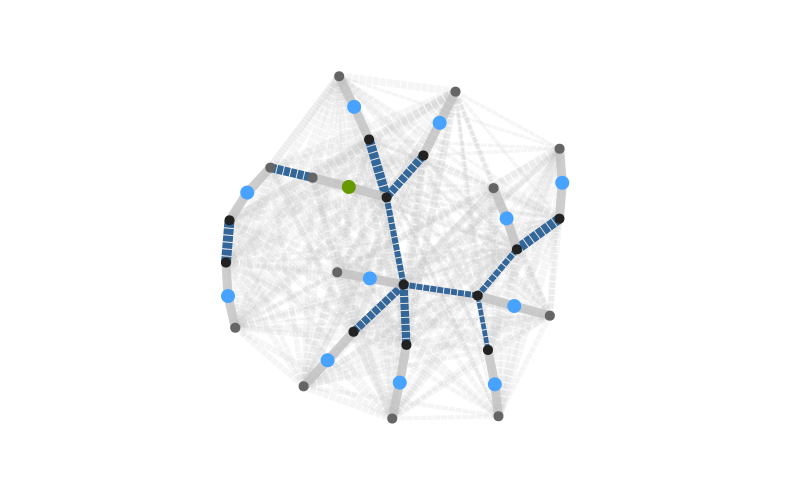
\includegraphics[width=0.7\textwidth]{figures/topo_chan_1}%
	\caption{Topology of the testnetwork with only channel 1 being used. Different colors indicate different channels}
      }
      \label{fig:topo_chan_1}
    \end{figure}
    
    \begin{figure}[h]
      \centerline{
	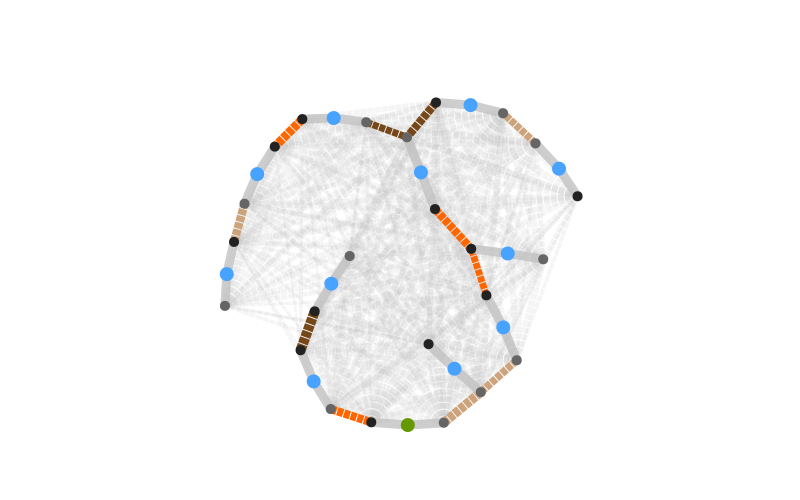
\includegraphics[width=0.7\textwidth]{figures/topo_chan_36_40_44}%
	\caption{Topology of the testnetwork with only channel 36,40,44 being used.}
      }
      \label{fig:topo_chan_36_40_44}
    \end{figure}

    \begin{figure}[h]
      \centerline{
	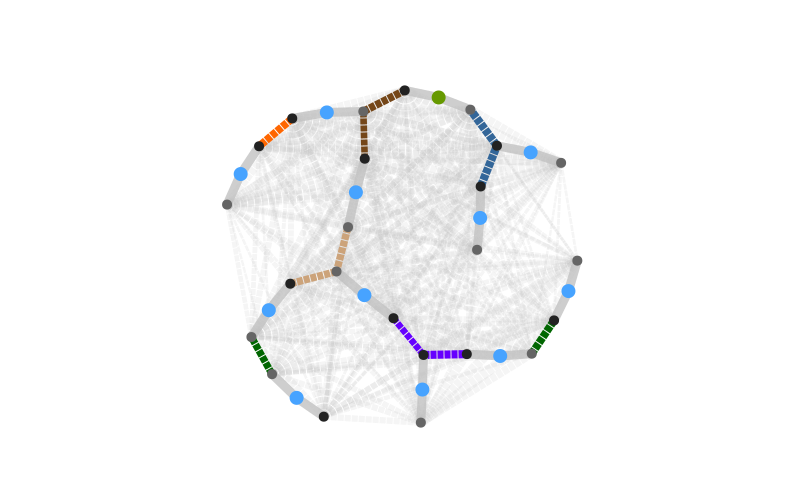
\includegraphics[width=0.7\textwidth]{figures/topo_chan_1_6_11_36_40_44}%
	\caption{Topology of the testnetwork with only channel 1,6,11,36,40,44 being used.}
      }
      \label{fig:topo_chan_1_6_11_36_40_44}
    \end{figure}
    
    \subsection{Characteristics}
    Due to the exceptional utilization of the 2.4 Ghz band in the area around the test arrangement, we had to carefully chose time and day
    for running the tests. We noticed a significant drop in radio usage for weekends and evenings and were able to schedule our tests in those timeframes.
    We additionally ran the testcases with two different settings to simulate the hidden station problem. Therefore we first set the radios to full power 
    resulting in a high connectivity between the nodes and on a second run decreased the transmit power as much as possbile to get a network with a smaller degree
    of interconnectivity.
\section{Results}
  \subsection{Expectations}
    We would expect a significant increase of data that has been able to transmit due to the usage of multiple collision domains the same one could
    expect by comparing a network hub, which as essentially just one collision domain and a network switch which has multiple domains and does not have
    to wait until the medium is free for sending again.
  \subsection{Actual Results}
    \begin{description}
     \item [Do the actual results diverge from the expected ones?]
     \item[Assessment of the base scenario]
      Base Scanario (uses only 1 Channel for all connections) pretty much broken by design -> Medium totally overloaded -> does not even scale to 3 APs in close proximity \newline
     \item[By how much is the solution better then before?]
      Despite being actually usable again, Traffic throughput is ~7-10 Times higher
    \end{description}
\section{Reflection on the requirements}
  How far does the solution meet the requirements?\newline
  \subsection{Increased Throughput}
    Definitely, see Diagrams \newline
  \subsection{Reduced Connectivity failures}
    Not tested, since test equippment lacks support for multi-flow/routing support (only bridged connections between APs) \newline
  \subsection{Multiple Radios utilized}
    Surely, with excess radios being usable for client connections \newline
  \subsection{Solution works within the perimeter}
    Absolutely, since we can compute CAA on central entity and works best for static scenarios \newline
  \subsection{Comply with Economic Restrictions}
    Runtime for Small scenarios (about 13 APs with about 500 Possible connections) on a modern system (fill in description of system) small -> <1 Second
    Estimate for bigger scenario missing (How do i correctly estimate that?)
\section{Reflection on related Work}
  Comparison to related Work algorithms\newline
  \subsection{Features of other Systems}
  \subsection{Features of our System}
\section{Discussion}
  \begin{description}
   \item [Checking the coloring and channel assignment after the algo run]
   this might not be the best place for this point, but serves just as a reminder.
   \item [What do the results mean?]
   Obviously it is useful to use mutliple channels for WDS system
   \item[What could'nt we measure?]
   What measurements are still missing:  run testcases for each parameter like formula,...
   Evaluate the redundant paths feature.
   Simulate the system with more accesspoints and various parameteres
  \end{description}
\chapter{Conclusion}
\section{Limitations}
  Where can't it be used?\newline
\section{Future Work}
  What is still to do?\newline
  Comparison to related work algorithms with actual measurements\newline



%%%%%%%%%%%%%%%%%%%%%%%%%%%%%%%%%%%%%%%%%%%%%%%%%%%%%%%%%%%%%
%% LITERATUR UND ANDERE VERZEICHNISSE
%%%%%%%%%%%%%%%%%%%%%%%%%%%%%%%%%%%%%%%%%%%%%%%%%%%%%%%%%%%%%
%% Ein kleiner Abstand zu den Kapiteln im Inhaltsverzeichnis (toc)
\ifnotdraft{
\addtocontents{toc}{\protect\vspace*{\baselineskip}}
\cleardoublepage
%% Literaturverzeichnis
\phantomsection % phantomsection wird benötigt, damit z.B. hyperref die richtige Seite verlinkt.
\addcontentsline{toc}{chapter}{Bibliography}
\nocite{*} %Auch nicht-zitierte BibTeX-Einträge werden angezeigt.
\bibliography{literature/literature.bib}%Eine Datei 'literatur.bib' wird hierfür benötigt.
\bibliographystyle{styles/acmurl}%Art der Ausgabe: plain / apalike / amsalpha / ...
}

%% Abbildungsverzeichnis
%\clearpage
%\addcontentsline{toc}{chapter}{List of Figures}
%\listoffigures

%% Tabellenverzeichnis
%\clearpage
%\addcontentsline{toc}{chapter}{List of Tables}
%\listoftables


%%%%%%%%%%%%%%%%%%%%%%%%%%%%%%%%%%%%%%%%%%%%%%%%%%%%%%%%%%%%%
%% ANHÄNGE
%%%%%%%%%%%%%%%%%%%%%%%%%%%%%%%%%%%%%%%%%%%%%%%%%%%%%%%%%%%%%
\appendix
\chapter{Appendix}

\section{List of Abbreviations}

\begin{acronym}[ABCDEFGH]
	\setlength{\itemsep}{-\parsep}
	
	\acro{ABC}{Alphabet}
\end{acronym}


\end{document}
